\documentclass{beamer}
\usepackage[T1]{fontenc} \usepackage{lmodern} \usepackage[utf8]{inputenc}
\usepackage[english]{babel} \usepackage{booktabs}
\usepackage{graphicx,subcaption} \usepackage{amssymb,amsmath}
\graphicspath{{figures/}}
\usepackage[citestyle=authoryear,bibstyle=authoryear,backend=biber,url=false,doi=false,isbn=false]{biblatex} \bibliography{refs}
\usepackage{hyperref}

% Make Adobe Reader use the RGB rendering model for pages with transparency.
\pdfpageattr{/Group << /S /Transparency /I true /CS /DeviceRGB>>}

\mode<presentation>{
	\usetheme{Malmoe}
	\usecolortheme{beaver}
	\setbeamertemplate{footline}[page number]
	\setbeamertemplate{navigation symbols}{}
}

%------------------------------------------------

\DeclareMathOperator*{\diag}{diag}
\DeclareMathOperator*{\argmin}{arg\,min}
\DeclareMathOperator*{\spn}{span}
\newcommand{\G}{\mathcal{G}}
\newcommand{\V}{\mathcal{V}}
\newcommand{\E}{\mathcal{E}}
\newcommand{\bO}{\mathcal{O}}
\newcommand{\R}{\mathbb{R}}

\newcommand{\good}[1]{{\color[rgb]{0.2,0.6,0.2}#1}}
\newcommand{\bad}[1]{{\color{red}#1}}
\newcommand{\txt}[1]{\hspace{.5cm} \text{#1} \hspace{.5cm}}
\newcommand{\define}[1]{\item{\usebeamercolor[fg]{enumerate item}#1}:}
\newcommand{\HRule}{{\usebeamercolor[bg]{subsection in head/foot} \rule{\linewidth}{0.5mm}}}

%------------------------------------------------

\begin{document}

\begin{frame}[plain]
	%\titlepage
	\begin{center}

		\textsc{\large A Network Tour of Data Science}\\
		\vspace{0.7cm}

		\HRule
		\vspace{0.65cm}
		{
			\usebeamercolor[fg]{frametitle}
			%\textsc{\Large Practical Informations}\\
			\textsc{\Large Concluding Remarks}\\
			%\textsc{\Large Laboratories}\\
			\vspace{0.4cm}
		}
		\HRule
		\vspace{1.0cm}

		\hspace{0.5cm}
		\begin{minipage}{0.4\linewidth}
			\footnotesize
			\textbf{Teachers} \\
			Pierre \textsc{Vandergheynst} \\
			Pascal \textsc{Frossard} \\
		\end{minipage}
		\begin{minipage}{0.4\linewidth}
			\footnotesize
			\textbf{Assistants} \\
			Michaël \textsc{Defferrard} \\
			Effrosyni \textsc{Simou} \\
			Hermina \textsc{Petric Maretić} \\
		\end{minipage}

		\vspace{0.7cm}
		\footnotesize EPFL LTS2 \& LTS4 laboratories\\
		\vspace{0.3cm}
		\footnotesize December 22, 2017

	\end{center}
\end{frame}

%------------------------------------------------

\begin{frame}
	\frametitle{Your remarks}
	Evaluations: Overall, I think this course is good.
	\footnote{48 answers out of 109 registered students.}
	\vfill
	\begin{itemize}
		\item 32\% strongly agree
		\vspace{0.5em}
		\item 51\% agree
		\vspace{0.5em}
		\item 11\% disagree
		\vspace{0.5em}
		\item  2\% strongly disagree
		\vspace{0.5em}
		\item  4\% no opinion
	\end{itemize}
\end{frame}

%------------------------------------------------

\begin{frame}
	\frametitle{Your remarks}
	% Don't touch remarks on teaching, not my area.
	\begin{itemize}
		\item No Deep Learning!
		\begin{itemize}
			\item \href{http://edu.epfl.ch/coursebook/en/deep-learning-EE-559}{Deep Learning, EE-559, François Fleuret}
			\item \href{https://edu.epfl.ch/coursebook/en/artificial-neural-networks-CS-456}{Artificial neural networks, CS-456, Wulfram Gerstner}
			\item Expand the part on DL with graphs?
		\end{itemize}
		\vfill
		\item Should we continue with tutorials / demos?
			\\ Assignments only? Exercises?
		\vfill
		\item Homeworks useful to assimilate the material.
		\vfill
		\item Start project earlier?
		\vfill
		\item Give feedback on the assignments earlier.
	\end{itemize}
\end{frame}

%------------------------------------------------

\begin{frame}
	\frametitle{My remarks}
	\begin{itemize}
		\item Engaged students.
		\vfill
		\item Interesting discussions, and solutions.
		\vfill
		\item Good job on the assignments! (so far ;)
		\vfill
		\item Looking forward to the project's presentations!
	\end{itemize}
\end{frame}

%------------------------------------------------

\begin{frame}
	\frametitle{Challenge}
	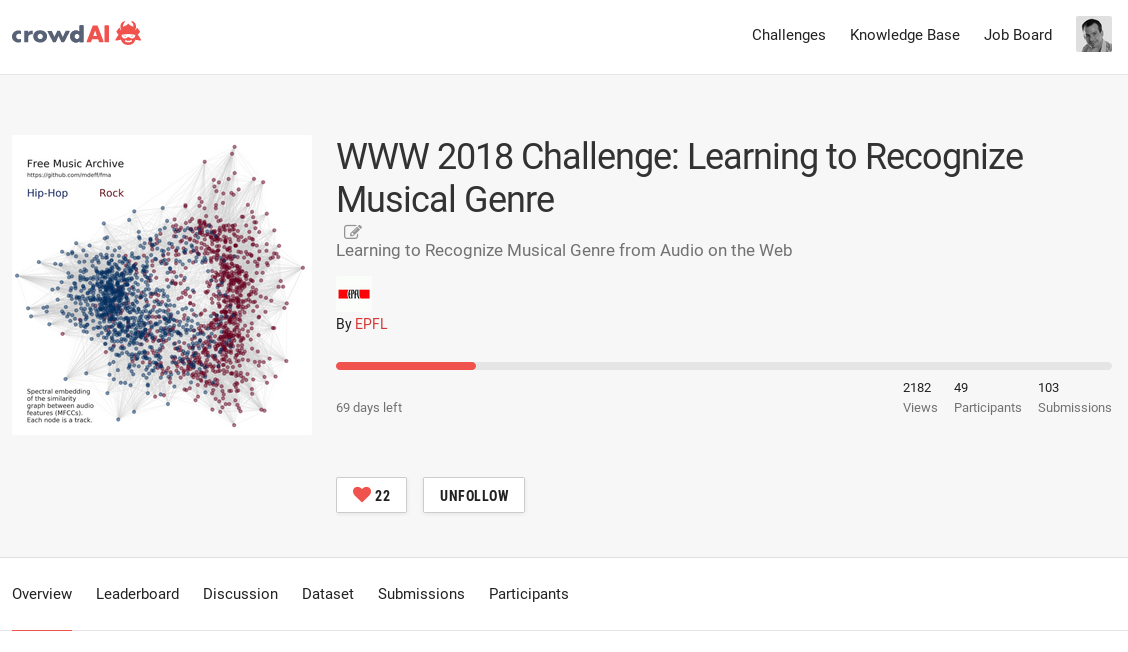
\includegraphics[width=\linewidth]{fma_challenge}
	\vfill
	\tiny
	\url{https://www.crowdai.org/challenges/www-2018-challenge-learning-to-recognize-musical-genre}
\end{frame}

%------------------------------------------------

\begin{frame}
	\frametitle{Projects}
	\begin{center}
		Always looking for talented people!
	\end{center}
	\vfill
	\begin{itemize}
		\item \href{https://lts2.epfl.ch/projects/67}{Deep learning on 3D point clouds for object detection}
			\\ {\footnotesize Master thesis}
			\\ {\footnotesize machine learning, graphs, real data}
		\vfill
		\item Work on the \href{https://github.com/mdeff/fma/}{FMA music dataset}
			\\ {\footnotesize Semester project or Master thesis}
			\\ {\footnotesize data exploration, machine learning}
		\vfill
		\item Help develop the \href{https://github.com/epfl-lts2/pygsp}{PyGSP}
			\\ {\footnotesize Semester project}
			\\ {\footnotesize scientific Python, software development and maintenance, open-source}
	\end{itemize}
\end{frame}

%------------------------------------------------

\begin{frame}
	\Huge{\centerline{Thanks for attending NTDS}}
	\vfill
	\Huge{\centerline{and}}
	\vfill
	\Huge{\centerline{Merry Christmas!}}
\end{frame}

%------------------------------------------------

\end{document}
